\documentclass[a4paper,titlepage]{article}
\usepackage[utf8]{inputenc}
\usepackage{fullpage}
\usepackage{indentfirst}
\usepackage[per-mode=symbol]{siunitx}
\usepackage{listings}
\usepackage{graphicx}
\usepackage{color}
\usepackage{amsmath}
\usepackage{array}
\usepackage[hidelinks]{hyperref}
\usepackage[format=plain,font=it]{caption}
\usepackage{subcaption}
\usepackage{standalone}
\usepackage[nottoc]{tocbibind}
\usepackage[noabbrev,capitalize,nameinlink]{cleveref}
\usepackage{listings}
\usepackage{xspace}
\usepackage{titlesec}
\usepackage[cache=false]{minted}
\usepackage{booktabs}
\usepackage{csvsimple}
\newcommand{\MATLAB}{\textsc{Matlab}\xspace}
\usepackage{siunitx}
\usepackage[super]{nth}
\usepackage[titletoc]{appendix}

% Custom commands
\newcommand\numberthis{\addtocounter{equation}{1}\tag{\theequation}}
\newcommand{\code}[1]{\texttt{#1}}
\newcolumntype{P}[1]{>{\centering\arraybackslash}p{#1}}

\setminted{linenos,breaklines,fontsize=auto}

%\titleformat*{\section}{\normalsize\bfseries}
%\titleformat*{\subsection}{\small\bfseries}
\renewcommand{\thesubsection}{\thesection.\alph{subsection}}
\providecommand*{\listingautorefname}{Listing}
\newcommand*{\Appendixautorefname}{Appendix}

%opening
\title{\textbf{ECSE 543: Numerical Methods} \\ Assignment 1}
\author{Wenjie Wei \\ 260685967}
\date{\today}

\begin{document}
	\sloppy
	\maketitle
	
	\tableofcontents
	
	
	\twocolumn
	
	\section{Introduction}
	
	All programs in this assignment are written and compiled with Python 3.6. This report is structured so that the individual problems are answered in respective sections. The python codes used to solve the assignment problems are attached in the appendices, with the file names labeled at the top of the code segments.
	
	\section{Choleski Decomposition}
		\subsection{Choleski Implementation}
			The implementation of Choleski decomposition is shown in Listing \ref{lst:choleski}. There are two methods defined in \mintinline{python}{choleski.py}: \mintinline{python}{check_choleski(A, b, x)} and \mintinline{python}{choleski_decomposition(A, b)}. The latter method takes two matrices \mintinline{python}{A} and \mintinline{python}{b} as arguments, and returns \mintinline{python}{x} as the computational result of the decomposition. The first method takes these three matrices as arguments, and performs matrix production to check the result of
			$$
				Ax = b
			$$ 
			The precision of the equality is set to 0.001, as the program may end up with results with uncertainties with a quantity level of $10^{-8}$.
			
		\subsection{Simple Tester Matrices}
			To examine the functionality of the implementation, some tester matrices are constructed. The first tester matrix has randomly chosen entries, under the condition that the matrix is a non-singular, symmetric, positive definite matrix:
			$$
				\begin{bmatrix}
					15 & -5 & 0 & -5 \\
					-5 & 12 & -2 & 0 \\
					0 & -2 & 6 & -2 \\
					-5 & 0 & -2 & 9
				\end{bmatrix} x =
				\begin{bmatrix}
					115\\
					22\\
					-51\\
					13
				\end{bmatrix}
			$$
			
			To ensure non-singularity and positiveness, the entries on the primary diagonal must be chosen to be positive, otherwise the program with raise errors, meaning that the matrix does not meet the requirement. If the Choleski Decomposition succeeds, the matrix is proven to be positive definite.
			\begin{figure}[!h]
				\centering
				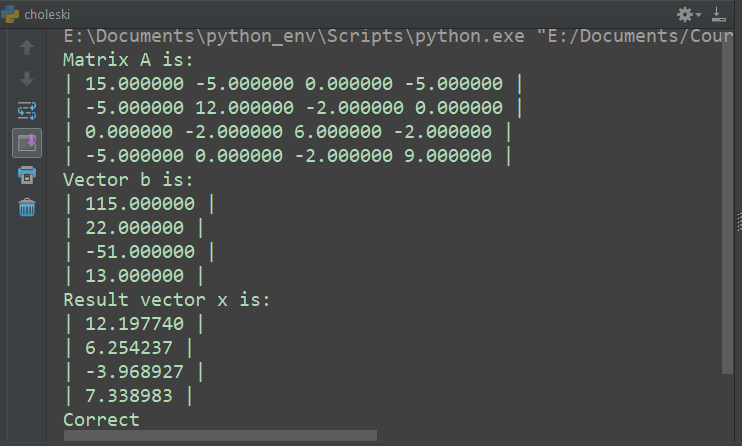
\includegraphics[width=\linewidth]{chol_1_result}
				\caption{Result of the First Choleski Decomposition Test}
				\label{chol_1_result}
			\end{figure}
		
			Figure \ref{chol_1_result} shows the result of the test of this certain tester matrix. This result is found to be correct by checking the dot product (which is implemented in file \mintinline{python}{matrix.py}) of matrix A and vector x. This result is also verified by \MATLAB using the back slash operator.
	
	\onecolumn
	\begin{appendices}
		
		\section{Code Listings} \label{appendix:code}
		
		\setminted{linenos,breaklines,fontsize=\footnotesize}
		
		\begin{center}
			\captionof{listing}{Custom matrix package (\texttt{matrix.py}).}
			\inputminted{python}{../matrix.py}
			\label{lst:matrices}
		\end{center}
		
		\begin{center}
			\captionof{listing}{Choleski decomposition (\texttt{choleski.py}).}
			\inputminted{python}{../choleski.py}
			\label{lst:choleski}
		\end{center}
		
		\begin{center}
			\captionof{listing}{Linear resistive networks (\texttt{linear\_networks.py}).}
			\inputminted{python}{../linearNetwork.py}
			\label{lst:linear_networks}
		\end{center}
		
	\end{appendices}
	

\end{document}